
\begin{document}

\chapter{Results}
\label{chapter:results}

This chapter summarizes the results in each user study and makes comparisons between a number of different studies. The results should provide insights into the reliability and accuracy of the tracking algorithm in different settings. In additiona, it would show the coordinates and joints that yield the most stable results during normal human activities.

\section{Accessing the data}
\label{sec:results_access_data}

The complete dataset and plots are publicly available at \url{https://github.com/cjw-charleswu/KinectMultiTrackDataset}

\section{Analysis}
\label{sec:results_analysis}

The analysis was done in Matlab 2015a. The analysis scripts are available at \url{https://github.com/cjw-charleswu/KinectMultiTrack/tree/master/Analysis}.

\subsection{Cleaning the data}
The logging data are post-processed for ease of plotting the results. The initial logging data, for all aforementioned studies, contain 244,527 rows and 87 columns in total. The final data for evaluation contain 243,550 rows and 87 columns. 977 rows are deleted for various reasons documented below.

There is also an error in code where a scenario id is logged incorrectly. In the second part of scenario 8, when the second participant is asked to walk around the first participant, the scenario id is falsely written as 4. This logging error is corrected by replacing all occurrences of scenario id 4 that are immediately after scenario id 8 and before scenario id 5, which is the next task in line for the participants.

The tracker time is stored as the server's current time in milliseconds. The times for each user task (scenario) are reset. The current timestamps refer to the amount of time passed in each scenario, for a particular Kinect configuration and experiment.

The timesalso converted from milliseconds to seconds. The joint coordinates are converted from meters to centimeters.

The studies are interested in the amount of coordinate differences between multiple skeletons after transformation during tracking. Thus, evaluation requires the joint positions of more than one skeletons (from different Kinect fields of view) at any given timestamp.

\section{Definitions}
\label{sec:results_definitions}

$\Delta x$, $\Delta y$, $\Delta z$, $\Delta d$, Avg., and Std. are defined as:

\begin{description}
  \item[\bm{$\Delta x$}] The distance, or difference, between the x coordinates of a joint of multiple skeletons representing the same person from different Kinects fields of view, expressed in centimeters.
  \item[\bm{$\Delta y$}] The distance, or difference, between the y coordinates of a joint of multiple skeletons representing the same person from different Kinects fields of view, expressed in centimeters.
  \item[\bm{$\Delta z$}] The distance, or difference, between the z coordinates of a joint of multiple skeletons representing the same person from different Kinects fields of view, expressed in centimeters.
  \item[\bm{$\Delta d$}] The distance, or difference, between the x, y, and z coordinates of a joint of multiple skeletons representing the same person from different Kinects fields of view, expressed in centimeters.
  \item[Avg.] Average (mean)
  \item[Std.] Standard deviation
\end{description}

These values quantify the amount of differences produced by the tracking algorithm when transforming multiple skeletons of the same person to a single Kinect field of view.

Coordinates and joints distances are defined as:

\begin{description}
  \item[Coordinates distances] The $\Delta x$, $\Delta y$, $\Delta z$, and $\Delta d$ distances averaged over a person's entire set of joints, expressed in centimeters.
  \item[Joints distances] The $\Delta x$, $\Delta y$, $\Delta z$, and $\Delta d$ distances for each of a person's joints, expressed in centimeters. 
\end{description}

\section{Structure}
\label{sec:results_structure}

There are three main results sections, one for each of the primary tasks, namely the Stationary, Steps, and Walk tasks. Each of these sections contains three basic visualizations showing the effects of the particular scenario on coordinates transformation errors when tracked with Kinects at different locations.

Each main section will begin with a figure showing changes in the average coordinates and joints distances with Parallel, 45$^{\circ}$ and 90$^{\circ}$ apart Kinects. The x asis will be the position of Kinect placement. The y axis will be the average coordinates distances, in terms of $\Delta x$, $\Delta y$, $\Delta z$, and $\Delta d$ (as defined in \ref{sec:results_definitions}). The figures will also entail the average coordinates distances over all of the Kinect placements.

The second figure will give more details about the average case shown in the previous figure. It will show changes in the average coordinates distances for each of the joint types. The x asis will be the joint type. The y axis will be the average joints distances, also in terms of $\Delta x$, $\Delta y$, $\Delta z$, and $\Delta d$.

Then, each section will finish with a table summarizing the actual values of the average coordinates distances for the presented task with each of the Kinect placements, as well as averaged over all different placements. The figures show how Kinect placements affect the average coordinates and joints distances during the Steps task.

At last, the results obtained from different scenarios and Kinect placements are compared. Figures will show the average coordinates and joints differences over time.

\section{Stationary}
\label{sec:results_stationary}

This section reports average coordinates and joints distances in the Stationary task with parallel, 45$^{\circ}$ and 90$^{\circ}$ apart Kinects.

The $\Delta d$ distance in the Stationary task with parallel Kinects is $3.52$ cm. The $\Delta d$ distance in the Stationary task with 45$^{\circ}$ apart Kinects is $3.95$ cm. The $\Delta d$ distance in the Stationary task with 90$^{\circ}$ apart Kinects is $11.39$ cm. The difference between the best and worst cases is $7.87$ cm. The average $\Delta d$ distance in the Stationary task over all Kinect placements is $7.9$,cm, with a standard deviation of $3.95$ cm.

\begin{figure}[!h]
  \centering

  \subfloat[Average coordinates distances in the Stationary task with Parallel, 45$^{\circ}$ and 90$^{\circ}$ apart Kinects.]{
      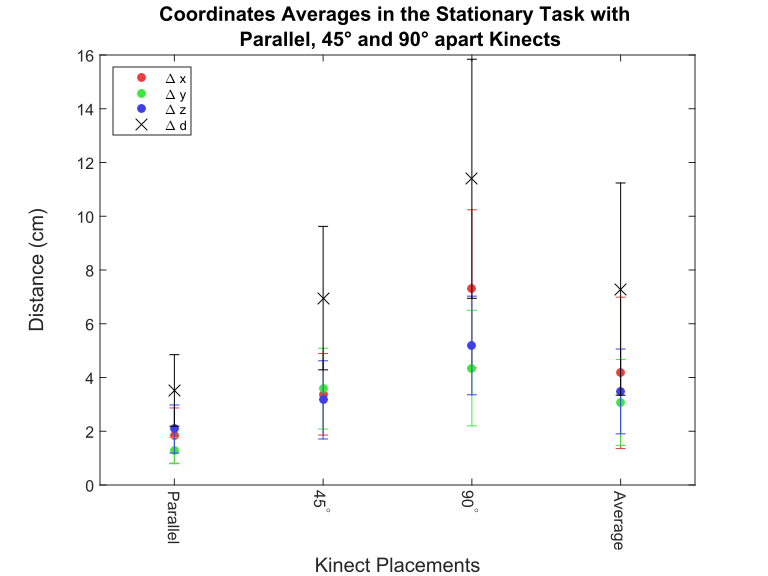
\includegraphics[width=0.50\linewidth]{figs/Coordinates_Task_Stationary}
      \label{fig:stationary_coordinates}
    }
    \subfloat[Average joints distances in the Stationary task averaged over Parallel, 45$^{\circ}$ and 90$^{\circ}$ apart Kinects.]{
      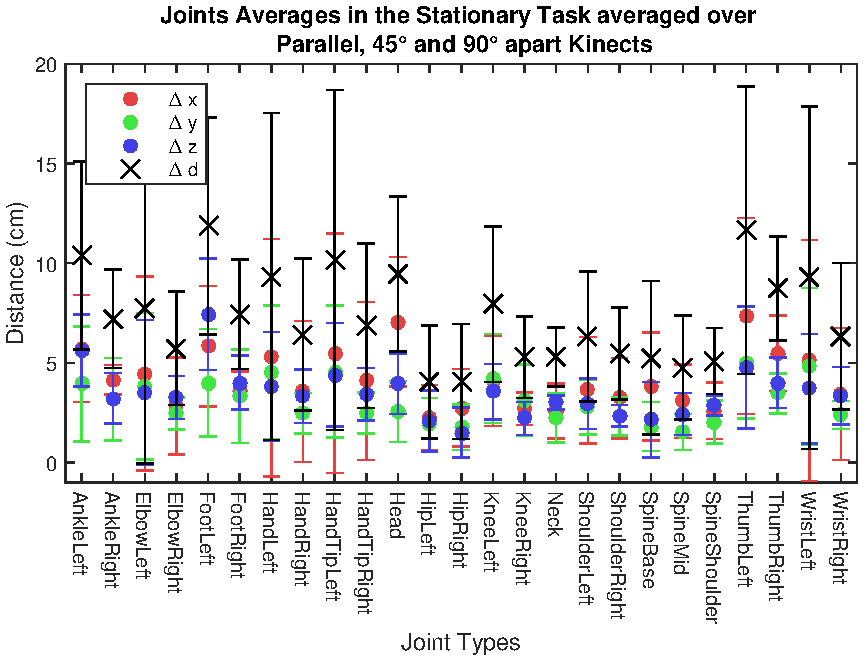
\includegraphics[width=0.50\linewidth]{figs/Joints_Task_Stationary}
      \label{fig:stationary_joints}
    }

  \caption{Plots showing the results in the Stationary task with different Kinect placements.}

  \label{fig:stationary_coordinates_joints}
\end{figure}

\begin{table}[!h]
\centering
  
  \begin{tabulary}{1.0\linewidth}{||c c c c c||} 
   \hline
   \textbf{Distances} & \textbf{Parallel} & \textbf{45$^{\circ}$} & \textbf{90$^{\circ}$} & \textbf{Average} \\ [0.5ex] 
   \hline\hline
   \textbf{Avg.} \bm{$\Delta x$} & 1.84 & 3.38 & 7.30 & 4.17 \\
   \hline
   \textbf{Std.} \bm{$\Delta x$} & 1.03 & 1.52 & 2.94 & 2.82 \\
   \hline
   \textbf{Avg.} \bm{$\Delta y$} & 1.28 & 3.59 & 4.35 & 3.07 \\
   \hline
   \textbf{Std.} \bm{$\Delta y$} & 0.49 & 1.50 & 2.15 & 1.60 \\
   \hline
   \textbf{Avg.} \bm{$\Delta z$} & 2.08 & 3.17 & 5.1917 & 3.48 \\
   \hline
   \textbf{Std.} \bm{$\Delta z$} & 0.89 & 1.45 & 1.84 & 1.58 \\
   \hline
   \textbf{Avg.} \bm{$\Delta d$} & 3.52 & 6.95 & 11.39 & 7.29 \\
   \hline
   \textbf{Std.} \bm{$\Delta d$} & 1.33 & 2.67 & 4.45 & 3.95 \\
   \hline
  \end{tabulary}
  
  \caption{Average coordinates distances in the Stationary task with Parallel, 45$^{\circ}$ and 90$^{\circ}$ Kinects, as well as the average case. The means and standard deviations for $\Delta x$, $\Delta y$, $\Delta z$, and $\Delta d$ are reported.}
  
  \label{table:stationary_coordinates_values}
\end{table}

\section{Steps}
\label{sec:results_steps}

This section reports average coordinates and joints distances in the Steps task with parallel, 45$^{\circ}$ and 90$^{\circ}$ apart Kinects.

The $\Delta d$ distance in the Steps task with parallel Kinects is $6.87$. The $\Delta d$ distance in the Steps task with 45$^{\circ}$ apart Kinects is $12.80$. The $\Delta d$ distance in the Steps task with 90$^{\circ}$ apart Kinects is $25.13$. The average $\Delta d$ distance in the Steps task over all Kinect placements is $14.93$, with a standard deviation of $9.32$.

\begin{figure}[!h]
  \centering

  \subfloat[Average coordinates distances in the Steps task with Parallel, 45$^{\circ}$ and 90$^{\circ}$ apart Kinects.]{
    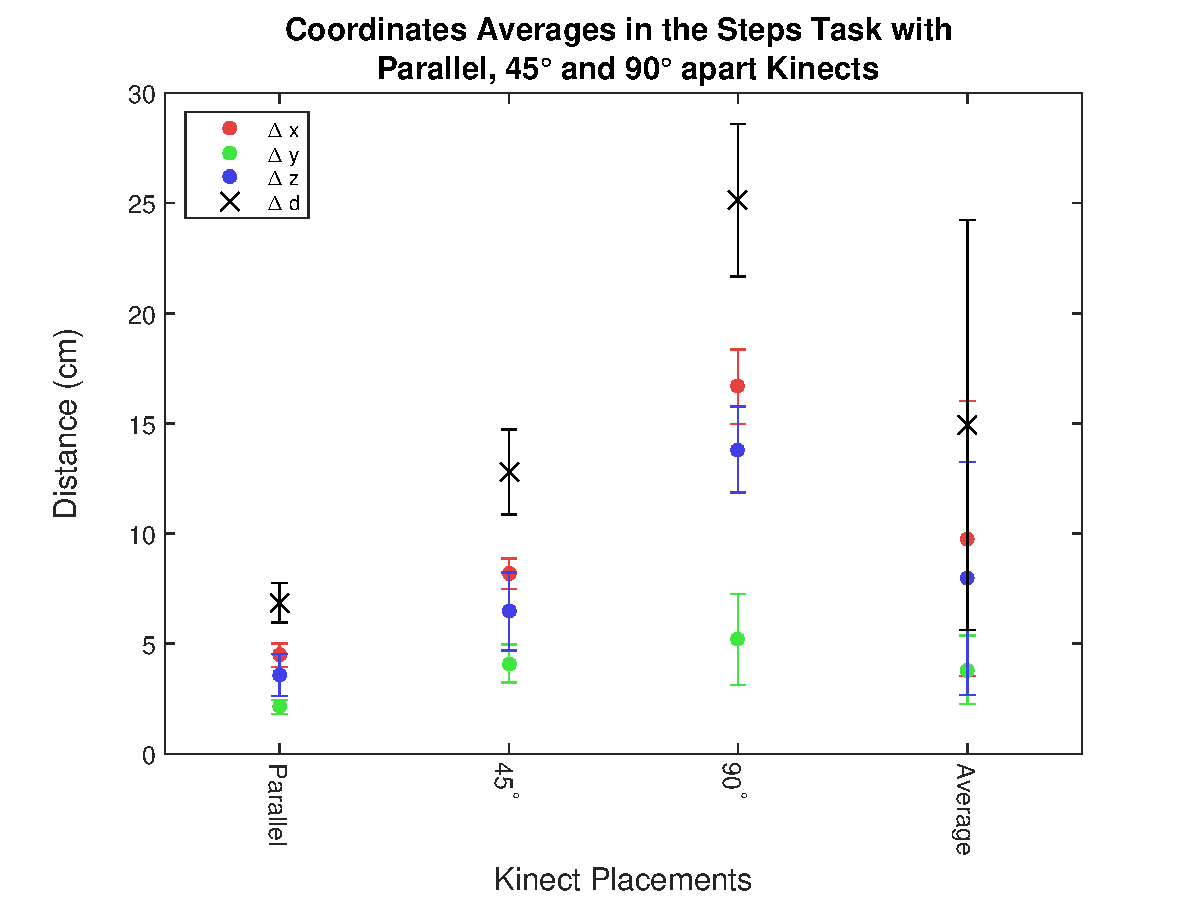
\includegraphics[width=0.5\linewidth]{figs/Coordinates_Task_Steps}
    \label{fig:steps_coordinates}
  }
  \subfloat[Average joints distances in the Steps task averaged over Parallel, 45$^{\circ}$ and 90$^{\circ}$ apart Kinects.]{
    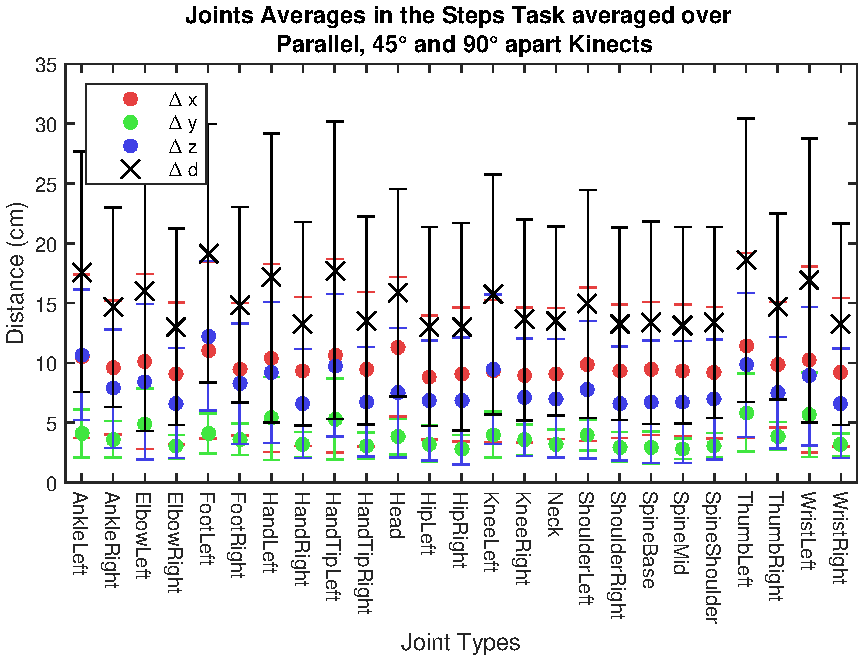
\includegraphics[width=0.5\linewidth]{figs/Joints_Task_Steps}
    \label{fig:steps_joints}
  }

  \caption{Plots showing the results in the Steps task with different Kinect placements.}

  \label{fig:steps_coordinates_joints}
\end{figure}

\begin{table}[!h]
\centering
  
  \begin{tabulary}{1.0\linewidth}{||c c c c c||} 
   \hline
   \textbf{Distances} & \textbf{Parallel} & \textbf{45$^{\circ}$} & \textbf{90$^{\circ}$} & \textbf{Average} \\ [0.5ex] 
   \hline\hline
   \textbf{Avg.} \bm{$\Delta x$} & 4.48 & 8.18 & 16.7 & 9.78 \\
   \hline
   \textbf{Std.} \bm{$\Delta x$} & 0.53 & 0.70 & 1.70 & 6.25 \\
   \hline
   \textbf{Avg.} \bm{$\Delta y$} & 2.13 & 4.11 & 5.20 & 3.81 \\
   \hline
   \textbf{Std.} \bm{$\Delta y$} & 0.32 & 0.86 & 2.07 & 1.56 \\
   \hline
   \textbf{Avg.} \bm{$\Delta z$} & 3.58 & 6.47 & 13.83 & 7.96 \\
   \hline
   \textbf{Std.} \bm{$\Delta z$} & 0.95 & 1.77 & 1.95 & 5.28 \\
   \hline
   \textbf{Avg.} \bm{$\Delta d$} & 6.87 & 12.80 & 25.13 & 14.93 \\
   \hline
   \textbf{Std.} \bm{$\Delta d$} & 0.90 & 1.92 & 3.46 & 9.32 \\
   \hline
  \end{tabulary}

  \caption{Average coordinates distances in the Steps task with Parallel, 45$^{\circ}$ and 90$^{\circ}$ Kinects, as well as the average case. The means and standard deviations for $\Delta x$, $\Delta y$, $\Delta z$, and $\Delta d$ are reported.}
  
  \label{table:steps_coordinates_values}
\end{table}

% 
% WALK
% 
\section{Walk}
\label{sec:results_walk}

This section reports average coordinates and joints distances in the Walk task with parallel, 45$^{\circ}$ and 90$^{\circ}$ apart Kinects.

The $\Delta d$ distance in the Walk task with parallel Kinects is $10.17$. The $\Delta d$ distance in the Walk task with 45$^{\circ}$ apart Kinects is $17.67$. The $\Delta d$ distance in the Walk task with 90$^{\circ}$ apart Kinects is $32.38$. The average $\Delta d$ distance in the Walk task over all Kinect placements is $20.07$, with a standard deviation of $11.30$.

\begin{figure}[!h]
  \centering

  \subfloat[Average coordinates distances in the Walk task with Parallel, 45$^{\circ}$ and 90$^{\circ}$ apart Kinects.]{
    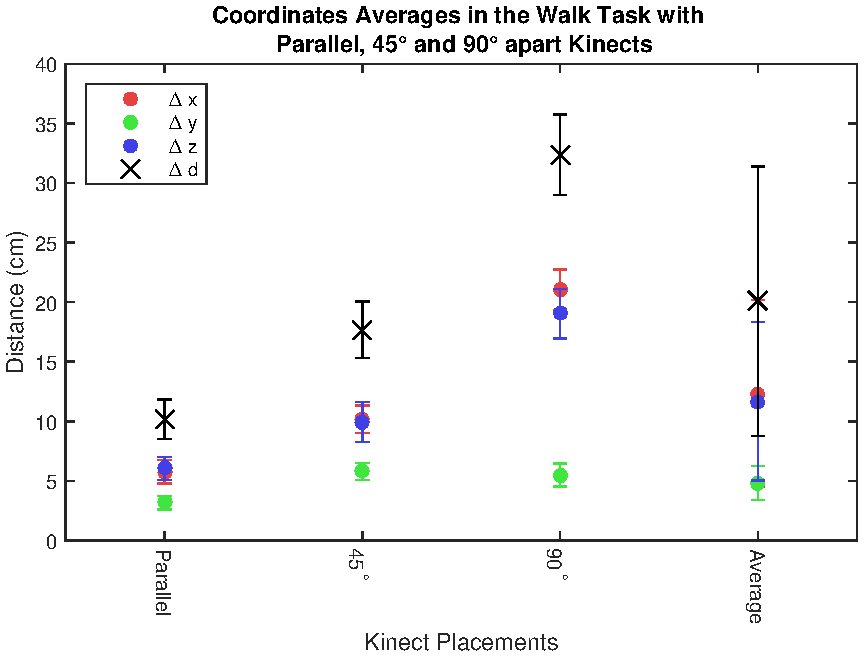
\includegraphics[width=0.5\linewidth]{figs/Coordinates_Task_Walk}
    \label{fig:walk_coordinates}
  }
  \subfloat[Average joints distances in the Walk task with Parallel, 45$^{\circ}$ and 90$^{\circ}$ apart Kinects.]{
    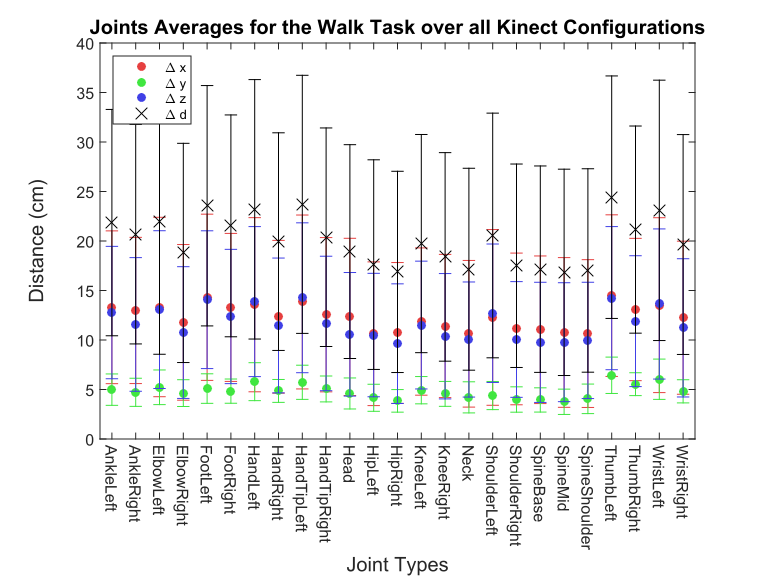
\includegraphics[width=0.5\linewidth]{figs/Joints_Task_Walk}
    \label{fig:walk_joints}
  }

  \caption{Plots showing the results in the Walk task with different Kinect placements.}

  \label{fig:walk_coordinates_joints}
\end{figure}

\begin{table}[!h]
  \centering

  \begin{tabulary}{1.0\linewidth}{||c c c c c||} 
   \hline
   \textbf{Distances} & \textbf{Parallel} & \textbf{45$^{\circ}$} & \textbf{90$^{\circ}$} & \textbf{Average} \\ [0.5ex] 
   \hline\hline
   \textbf{Avg.} \bm{$\Delta x$} & 5.76 & 10.18 & 21.02 & 12.32 \\
   \hline
   \textbf{Std.} \bm{$\Delta x$} & 0.97 & 1.16 & 1.73 & 7.85 \\
   \hline
   \textbf{Avg.} \bm{$\Delta y$} & 3.17 & 5.78 & 5.47 & 4.81 \\
   \hline
   \textbf{Std.} \bm{$\Delta y$} & 0.57 & 0.70 & 0.96 & 1.42 \\
   \hline
   \textbf{Avg.} \bm{$\Delta z$} & 6.04 & 9.94 & 19.03 & 11.67 \\
   \hline
   \textbf{Std.} \bm{$\Delta z$} & 0.95 & 1.69 & 2.07 & 6.67 \\
   \hline
   \textbf{Avg.} \bm{$\Delta d$} & 10.17 & 17.67 & 32.38 & 20.07 \\
   \hline
   \textbf{Std.} \bm{$\Delta d$} & 1.64 & 2.37 & 3.38 & 11.30 \\
   \hline
  \end{tabulary}

  \caption{Average coordinates distances in the Walk task with Parallel, 45$^{\circ}$ and 90$^{\circ}$ Kinects, as well as the average case. The means and standard deviations for $\Delta x$, $\Delta y$, $\Delta z$, and $\Delta d$ are reported.}
  
  \label{table:walk_coordinates_values}
\end{table}

% 
% STATIONARY, STEPS, WALK
% 
\section{Stationary, Steps, Walk}
\label{sec:results_stationary_steps_walk}

This section summarizes the results in the Stationary, Steps, and Walk tasks with Parallel, 45$^{\circ}$ and 90$^{\circ}$ apart Kinects.

Figure \ref{fig:results_three_coordinates_joints} shows two different plots. Firstly, it shows the average coordinates and joints distances in the Stationary, Steps, and Walk tasks averaged over different Kinect placements (Parallel, 45$^{\circ}$ and 90$^{\circ}$ apart Kinects). The reverse is also shown. The figure also shows the average coordinates and joints distances with Parallel, 45$^{\circ}$ and 90$^{\circ}$ apart Kinects averaged over different tasks (Stationary, , Steps, and Walk). The figure shows how the complexity of tasks and the placement of the Kinects, respectively, affect the accuracy of the tracking algorithm.

\begin{figure}[!h]
  \centering

  \subfloat[Average coordinates distances in the Stationary, Steps, and Walk tasks averaged over Parallel, 45$^{\circ}$ and 90$^{\circ}$ apart Kinects.]{

    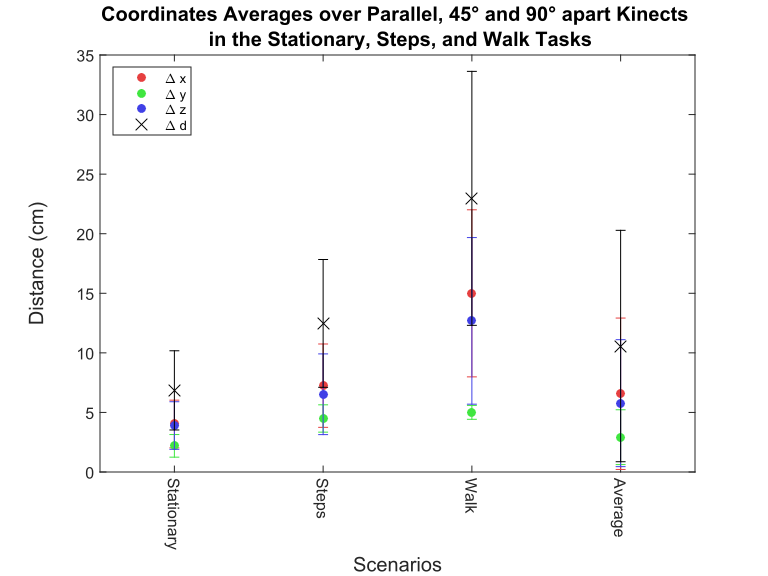
\includegraphics[width=0.5\linewidth]{figs/Coordinates_Kinect_All}
  
  }
  \subfloat[Average joints distances in the Stationary, Steps, and Walk tasks averaged over Parallel, 45$^{\circ}$ and 90$^{\circ}$ apart Kinects.]{
  
    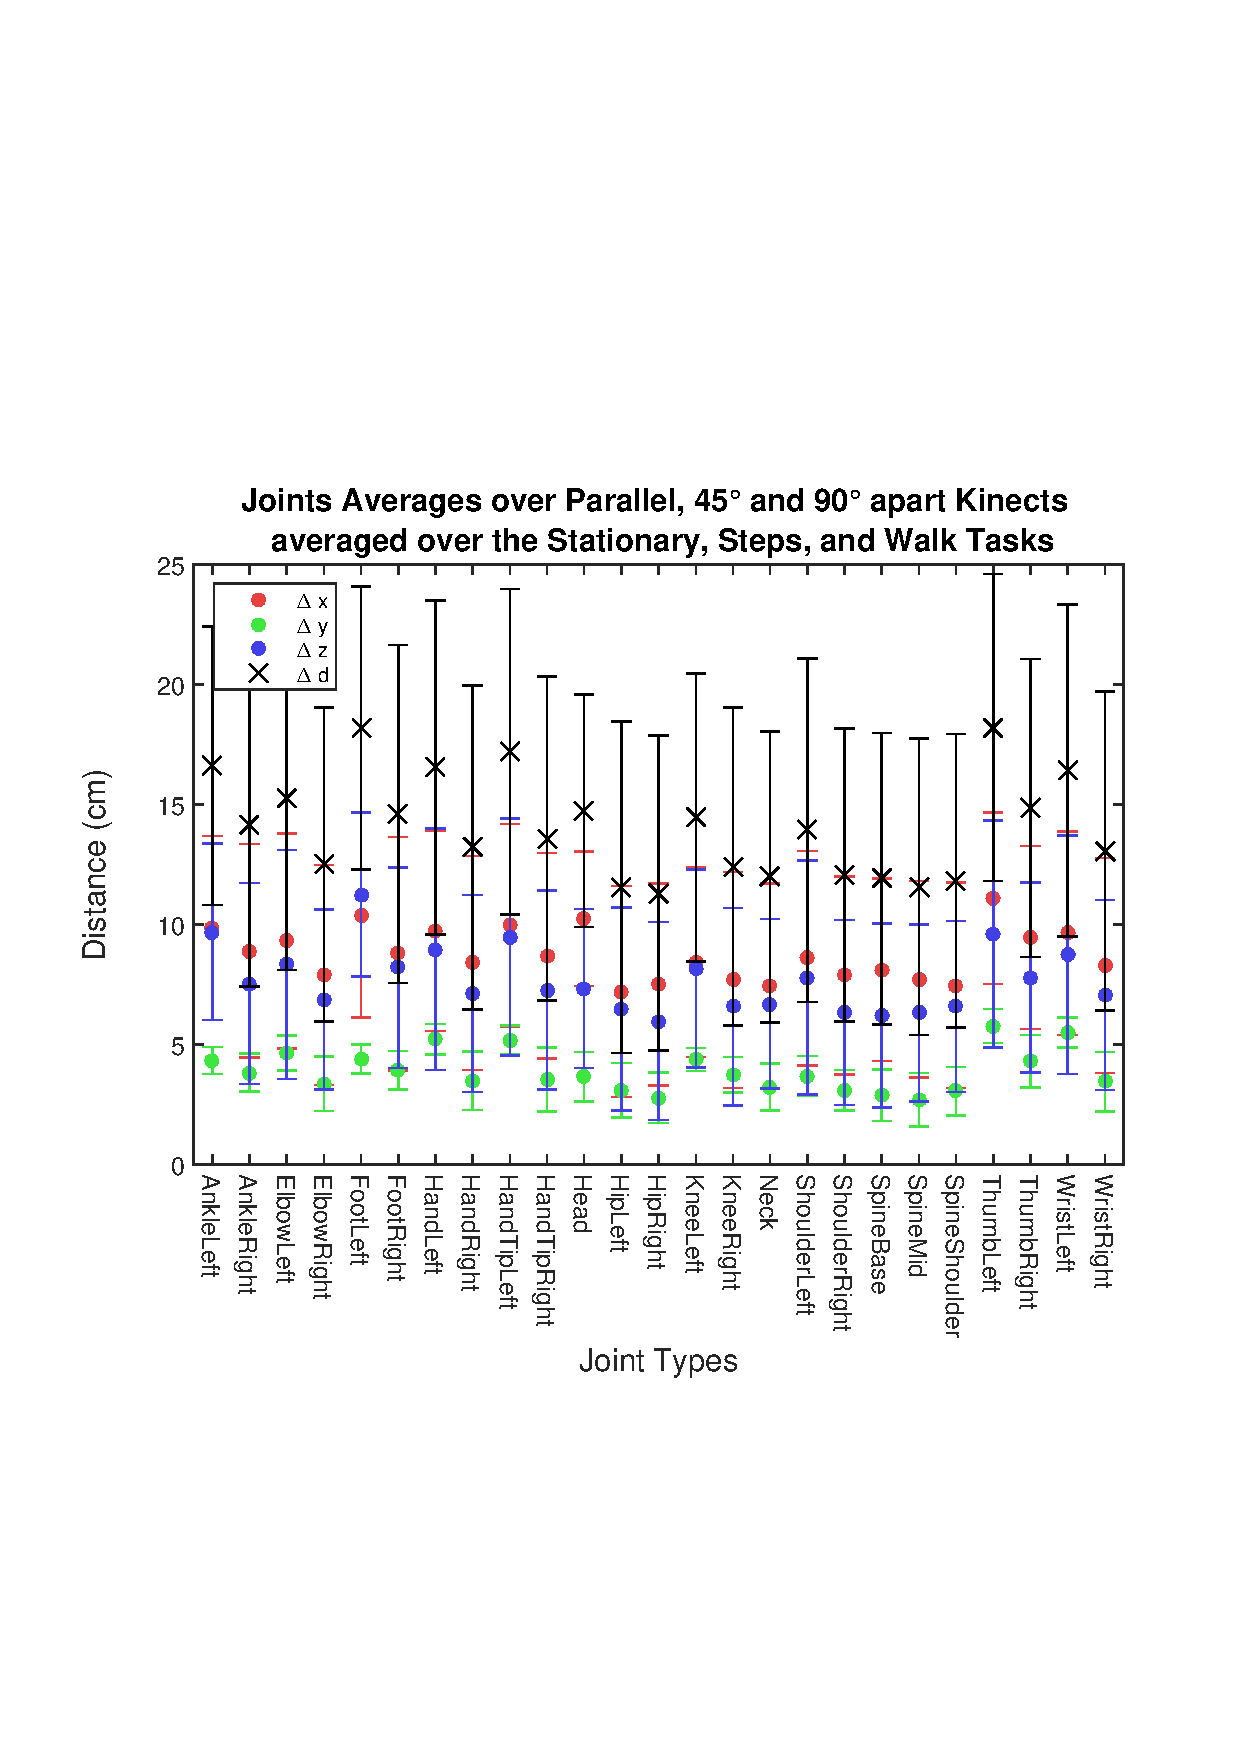
\includegraphics[width=0.5\linewidth]{figs/Joints_Kinect_All}
  
  } \\
    \subfloat[Average coordinates distances with Parallel, 45$^{\circ}$ and 90$^{\circ}$ apart Kinects averaged over Stationary, Steps, and Walk tasks.]{
  
    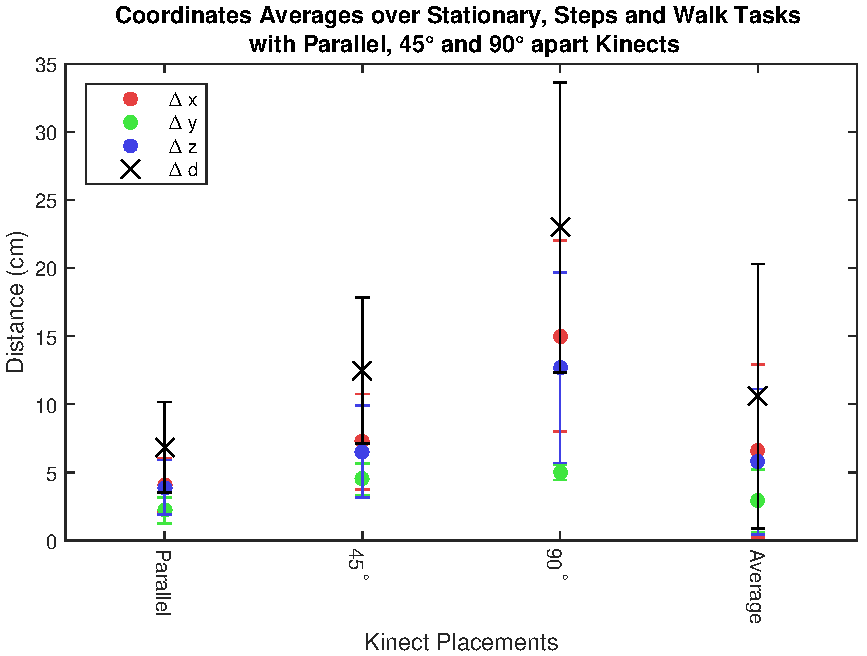
\includegraphics[width=0.5\linewidth]{figs/Coordinates_Task_All}
  
  }
  \subfloat[Average joints distances with Parallel, 45$^{\circ}$ and 90$^{\circ}$ apart Kinects averaged over Stationary, Steps, and Walk tasks.]{
  
    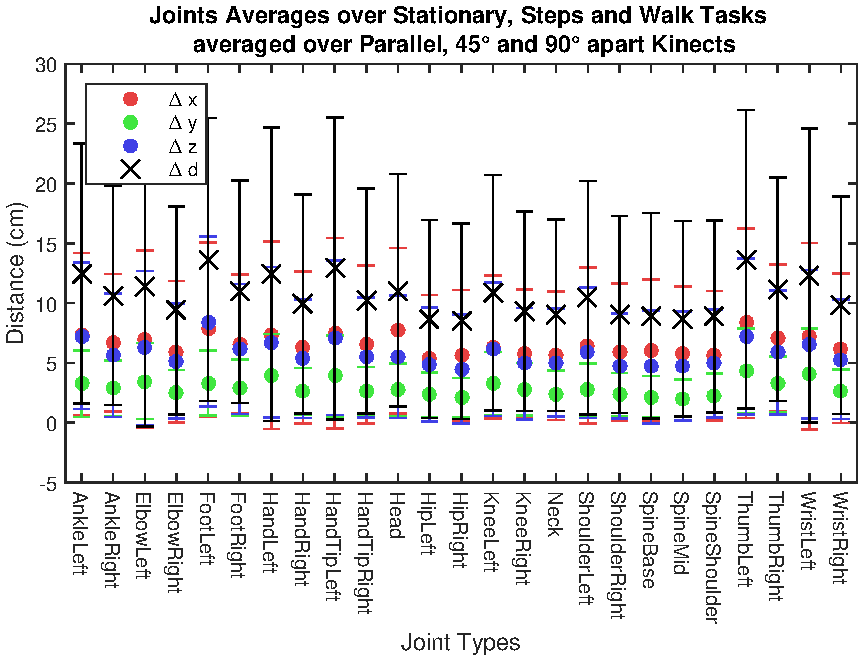
\includegraphics[width=0.5\linewidth]{figs/Joints_Task_All}
  
  }

  \caption{Plots showing the overall results in the Stationary, Steps, and Walk tasks with different Kinect placements.}

  \label{fig:results_three_coordinates_joints}
\end{figure}

\begin{table}[!h]
  \centering

  \subfloat[caption]{
    \begin{tabulary}{0.5\linewidth}{||c c c c c||} 
    \hline
    \textbf{Distances} & \textbf{Stationary} & \textbf{Steps} & \textbf{Walk} & \textbf{Average} \\ [0.5ex] 
    \hline\hline
    \textbf{Avg.} \bm{$\Delta x$} & 4.17 & 9.78 & 12.32 & 8.76 \\
    \hline
    \textbf{Std.} \bm{$\Delta x$} & 2.82 & 6.25 & 7.85 & 4.17 \\
    \hline
    \textbf{Avg.} \bm{$\Delta y$} & 3.07 & 3.81 & 4.81 & 3.90 \\
    \hline
    \textbf{Std.} \bm{$\Delta y$} & 1.60 & 1.56 & 1.42 & 0.87 \\
    \hline
    \textbf{Avg.} \bm{$\Delta z$} & 3.48 & 7.96 & 11.67 & 7.70 \\
    \hline
    \textbf{Std.} \bm{$\Delta z$} & 1.57 & 5.28 & 6.67 & 4.10 \\
    \hline
    \textbf{Avg.} \bm{$\Delta d$} & 7.29 & 14.93 & 20.07 & 14.10 \\
    \hline
    \textbf{Std.} \bm{$\Delta d$} & 3.95 & 9.32 & 11.30 & 6.43 \\
    \hline
    \end{tabulary} 
  }
  \subfloat[caption]{
    \begin{tabulary}{0.5\linewidth}{||c c c c c||} 
    \hline
    \textbf{Distances} & \textbf{Parallel} & \textbf{45$^{\circ}$} & \textbf{90$^{\circ}$} & \textbf{Average} \\ [0.5ex] 
    \hline\hline
    \textbf{Avg.} \bm{$\Delta x$} & 4.03 & 7.25 & 15.00 & 6.57 \\
    \hline
    \textbf{Std.} \bm{$\Delta x$} & 2.00 & 3.50 & 7.00 & 6.35 \\
    \hline
    \textbf{Avg.} \bm{$\Delta y$} & 2.19 & 4.49 & 5.01 & 2.92 \\
    \hline
    \textbf{Std.} \bm{$\Delta y$} & 0.95 & 1.15 & 0.58 & 2.30 \\
    \hline
    \textbf{Avg.} \bm{$\Delta z$} & 3.90 & 6.53 & 12.68 & 5.78 \\
    \hline
    \textbf{Std.} \bm{$\Delta z$} & 2.00 & 3.39 & 6.99 & 5.33 \\
    \hline
    \textbf{Avg.} \bm{$\Delta d$} & 6.85 & 12.47 & 22.97 & 10.57 \\
    \hline
    \textbf{Std.} \bm{$\Delta d$} & 3.32 & 5.36 & 10.66 & 9.71 \\
    \hline
    \end{tabulary}  
  }

  \caption{Table showing coordinates distances in the Walk task with Parallel, 45$^{\circ}$ and 90$^{\circ}$ Kinects, as well as the average case. The means and standard deviations for $\Delta x$, $\Delta y$, $\Delta z$, and $\Delta d$ are reported.}
  
  \label{table:results_three_coordinates_values}
\end{table}

\section{Obstacle}
\label{sec:results_obstacle}

\section{Interactions}
\label{sec:results_interactions}

\section{Overall}
\label{sec:results_overall}

\begin{figure}[!htb]
  \centering

  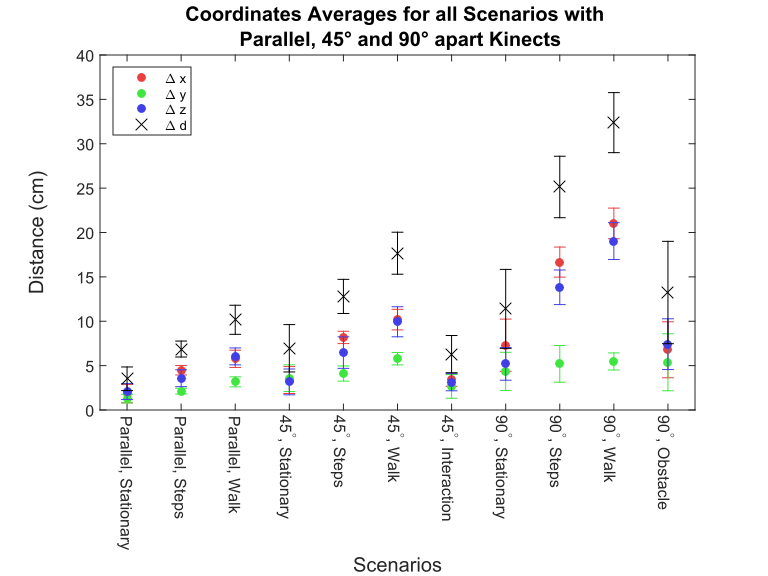
\includegraphics[width=1.0\linewidth]{figs/Coordinates_All}

  \caption{Plot showing the overall results for all scenarios in the studies}

  \label{fig:results_overall}
\end{figure}

\begin{table}[!h]
  \centering

  \begin{tabulary}{0.5\linewidth}{||c c c c c||} 
  \hline
  \textbf{Setup} & Avg. $\Delta x$ & Avg. $\Delta y$ & Avg. $\Delta z$ & Avg. $\Delta d$ \\ [0.5ex] 
  \hline\hline
  \textbf{Parallel, Stationery} & 1.84 & 3.38 & 7.30 & 4.17 \\
  \hline
  \textbf{Parallel, Steps} $\Delta y$ & 0.49 & 1.50 & 2.15 & 1.60 \\
  \hline
  \textbf{Parallel, Walk} $\Delta y$ & 0.49 & 1.50 & 2.15 & 1.60 \\
  \hline
  \textbf{45$^{\circ}$, Stationery} & 1.03 & 1.52 & 2.94 & 2.82 \\
  \hline
  \textbf{45$^{\circ}$, Steps} & 0.89 & 1.45 & 1.84 & 1.58 \\
  \hline
  \textbf{45$^{\circ}$, Walk} & 0.89 & 1.45 & 1.84 & 1.58 \\
  \hline
  \textbf{45$^{\circ}$, Interaction} & 0.89 & 1.45 & 1.84 & 1.58 \\
  \hline
  \textbf{90$^{\circ}$, Stationery} & 1.28 & 3.59 & 4.35 & 3.07 \\
  \hline
  \textbf{90$^{\circ}$, Steps} & 3.52 & 6.95 & 11.39 & 7.29 \\
  \hline
  \textbf{90$^{\circ}$, Walk} & 3.52 & 6.95 & 11.39 & 7.29 \\
  \hline
  \textbf{90$^{\circ}$, Obstacle} & 1.33 & 2.67 & 4.45 & 3.95 \\
  \hline
  \end{tabulary}
  
  \caption{Table showing the overall average coordinates distances}
  
  \label{table:overall_coordinates_values}
\end{table}

\end{document}
